% resume.tex
%
% Omid Mashayekhi

\documentclass[letterpaper,10pt]{article}

%-----------------------------------------------------------
\usepackage{enumitem}
\usepackage{graphicx}
\usepackage{textpos}
\usepackage[empty]{fullpage}
\usepackage[colorlinks=true, urlcolor=blue]{hyperref}
\raggedbottom
\raggedright
\setlength{\tabcolsep}{0in}

% Adjust margins to 0.5in on all sides
\addtolength{\oddsidemargin}{-0.5in}
\addtolength{\evensidemargin}{-0.5in}
\addtolength{\topmargin}{-0.5in}
\addtolength{\textheight}{1.0in}
\addtolength{\textwidth}{1.0in}

%-----------------------------------------------------------
%Custom commands

\newcommand{\heading}[1] {
  {\large
    \begin{minipage}
    {\textwidth}
    {\textbf{#1}}
    \end{minipage}
  }
  \begin{center}
  \vspace{-15pt}
  \line(1,0){520}
  \end{center}
}


\newcommand{\template}[2]{
\begin{tabular*}{7.0in}{l@{\extracolsep{\fill}}r}
		#1 & \textit{#2} \\
\end{tabular*}\vspace{-1pt}}

\newcommand{\templatex}[4]{
\begin{tabular*}{7.0in}{l@{\extracolsep{\fill}}r}
		\textbf{#1} & #2 \\
		\textit{~~~#3} & \textit{#4} \\
\end{tabular*}\vspace{-1pt}}

\newcommand{\templatexx}[6]{
\begin{tabular*}{7.0in}{l@{\extracolsep{\fill}}r}
		\textbf{#1} & #2 \\
		\textit{~~~#3} & \textit{#4} \\
		\textit{~~~#5} & \textit{#6} \\
\end{tabular*}\vspace{-1pt}}

\newcommand{\templatexxx}[8]{
\begin{tabular*}{7.0in}{l@{\extracolsep{\fill}}r}
		\textbf{#1} & #2 \\
		\textit{~~~#3} & \textit{#4} \\
		\textit{~~~#5} & \textit{#6} \\
		\textit{~~~#7} & \textit{#8} \\
\end{tabular*}\vspace{-1pt}}

%-----------------------------------------------------------


\begin{document}

\centering

\textbf{\LARGE Omid Mashayekhi}

\setlength{\TPHorizModule}{10pt} %controls horizontal movements
\setlength{\TPVertModule}{10pt}  %controls vertical movements

\begin{textblock}{4}(1,0)
\begin{tabular}{lr}
\textbf{Address:} & Gates 284, Stanford Univ.\\
                  & Stanford, CA 94305\\
\end{tabular}

\end{textblock}

\begin{textblock}{4}(37,0)
\begin{tabular}{lr}
E-Mail:     & 
\includegraphics[width=1.2in]{email.png}\\
% E-Mail    & omidm@stanford.edu\\

Cell Phone: & 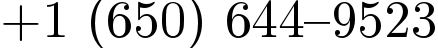
\includegraphics[width=1in]{cell-phone.png}\\
% Cell Phone: & +1 (650) 644--9523\\

Website:    & \href{http://www.stanford.edu/~omidm}{\url{www.stanford.edu/~omidm}}\\
\end{tabular}
\end{textblock}

\vspace{30pt}





\heading{Education}

\begin{tabular*}{7.0in}{l@{\extracolsep{\fill}}r}
\textbf{\large Stanford University}  \color{blue}{\footnotesize (expected graduation: June 2017)} & Stanford, CA \\
~~~\textbf{Ph.D.} in Electrical Engineering, Cloud Computing    & Winter 2013 - Present\\
~~~\textbf{Ph.D. Minor} in Computer Science, Systems Track       & Winter 2013 - Present\\
~~~\textbf{M.Sc.} in Electrical Engineering, Networking Systems & Fall 2011 - Spring 2013\\
\end{tabular*}

\vspace{5pt}

\begin{tabular*}{7.0in}{l@{\extracolsep{\fill}}r}
\textbf{Sharif University of Technology} & Tehran, Iran\\
~~~\textbf{B.Sc.} in Electrical Engineering, Communication Systems & Fall 2007 - Spring 2011\\
\end{tabular*}

\vspace{5pt}





\heading{Experience}

\begin{tabular*}{7.0in}{l@{\extracolsep{\fill}}r}
\textbf{Internship at bebop Inc.}  & Los Altos, CA \\
~~~Back-end engineer working on developing a low latency data store. &  Summer 2015\\
\end{tabular*}

\vspace{5pt}

\begin{tabular*}{7.0in}{l@{\extracolsep{\fill}}r}
\textbf{RA at Stanford Information Networks Group (SING)}  & Stanford University\\
~~~Diverse projects from cloud computing and graphical simulations to full duplex radio. & Fall 2011 - Present\\
% ~~~\textbf{Nimbus}: cloud computing framework for low latency data analytics and HPC applications. & \\
% ~~~(for more information visit: \href{http://nimbus.stanford.edu}{nimbus.stanford.edu}) & \\
% ~~~\textbf{Janus}:  &  \\
\end{tabular*}
	
\vspace{5pt}

\begin{tabular*}{7.0in}{l@{\extracolsep{\fill}}r}
\textbf{Internship at Cisco Systems }  & San Jose, CA \\
~~~Software engineer at Wireless Networking Business Unit (WNBU). & Summer 2012 \\
\end{tabular*}
	
\vspace{5pt}
	
\begin{tabular*}{7.0in}{l@{\extracolsep{\fill}}r}
\textbf{Teaching Experience} & Stanford University \\
~~~Course Assistant in CS344C, Cloud Simulation Systems. & Spring 2013 \\
\end{tabular*}
	
\vspace{5pt}

\begin{tabular*}{7.0in}{l@{\extracolsep{\fill}}r}
\textbf{RA at Advanced Communications Research Institute (ACRI) }  & Sharif University \\
~~~Research in power estimation and coding techniques for CDMA systems & Spring 2009 - Summer 2011 \\
\end{tabular*}
	
\vspace{5pt}





\heading{Selected Projects}

\begin{itemize}[noitemsep,topsep=0pt, leftmargin=.5cm, rightmargin=.5cm]

\item[]
\textbf{Nimbus Project:}
cloud computing framework for fast data analytics and HPC applications.
(\href{http://nimbus.stanford.edu}{nimbus.stanford.edu}).

\vspace{5pt}

\item[]
\textbf{Janus Project:}
centralized MAC protocol for full duplex radio that realizes double capacity.

\vspace{5pt}

\item[]
\textbf{Predicting x86 Runtime:}
supervised learning algorithms to predict serialized x86 programs runtime. 


\vspace{5pt}


\item[]
\textbf{Packet Classification in Presence of Wildcard:}
scalable, memory efficient, software-based algorithm.
	
\vspace{5pt}

\item[]
\textbf{OpenFlow Controller for DCell:}
simulating DCell topology for data centers using Mininet OpenFlow controller.
	
\end{itemize}

\vspace{5pt}





\heading{Papers}

\begin{itemize}[noitemsep,topsep=0pt, leftmargin=.5cm, rightmargin=.5cm]


\item[]
\textbf{O. Mashayekhi}, H. Qu, C. Shah, P. Levis
"Scalable, Fast Cloud Computing with Execution Templates",
arXiv:1606.01972 [cs.DC], 2016


\vspace{5pt}

\item[]
\textbf{O. Mashayekhi}, C. Shah, H. Qu, P. Levis
"Distributed Graphical Simulation in the Cloud",
arXiv:1606.01966 [cs.DC], 2016

\vspace{5pt}

\item[]
H. Qu, \textbf{O. Mashayekhi}, D. Terei, P. Levis,
"Canary: A Scheduling Architecture for High Performance Cloud Computing",
Stanford CSTR 2016-01, 2016.


\vspace{5pt}

\item[]
J. Y. Kim, \textbf{O. Mashayekhi}, H. Qu, M. Kazandjieva, and P. Levis,
"Janus: A Novel MAC Protocol for Full Duplex Radio",
Stanford CSTR 2013-02, 2013.

\vspace{5pt}

\item[]
\textbf{O. Mashayekhi}, and F. Marvasti,
"Uniquely Decodable Codes with Fast Decoder for Overloaded Synchronous CDMA Systems",
\textit{IEEE Transactions on Communication}, vol. 60, no. 11, pp. 3145-3149, November 2012.

\end{itemize}

\vspace{5pt}





\heading{Patents}

\begin{itemize}[noitemsep,topsep=0pt, leftmargin=.5cm, rightmargin=.5cm]
\item[]
{\textbf{O. Mashayekhi}, and F. Marvasti, "Uniquely Decodable Codes and Decoder for Overloaded Synchronous CDMA Systems", U.S. patent application no. 13,082,084, April 7/2011.}
	\end{itemize}

\vspace{5pt}





% \heading{Submissions}
% 	\begin{itemize}
% 		\item{J. Y. Kim, \textbf{O. Mashayekhi}, H. Qu, M. Kazandjieva, and P.
%       Levis, "Media Access in Full Duplex Wireless Networks". Submitted to
%         \textit{Infocomm'14}, July 2013.}
% 		\item{D. Nashtaali, \textbf{O. Mashayekhi}, P. Pad, R. Moghadasi, and F. Marvasti, "New Power Estimation Methods for Highly Overloaded Synchronous CDMA Systems". Submitted to \textit{IEEE Transactions on Wireless Communications}.}
% 	\end{itemize}

%	\template{\large \textbf{Conference Paper}}{~}
%	\begin{itemize}
%		\item{D. Nashtaali, \textbf{O. Mashayekhi}, P. Pad, R. Moghadasi, and F. Marvasti, "Optimum and Suboptimum Power Estimation for Highly Overloaded Synchronous CDMA Systems". Submitted to \textit{ISIT '11}, Feb. 2011.}
%	\end{itemize}



%\heading{Work Experience}
%\begin{itemize}
%
%\item \template{Working on Multi-User Detection and Channel Estimation, "Baregheh Communication" corporation.} {Summer 2010}
%
%\item \template{Pre-University consultant in Salam high school.} {Summer 2009}
%
%\item \template{Calculus teacher of Energy high school for pre-university students.}{Summer 2007}
%
%\end{itemize}
%
%



\heading{Honors and Awards}
\begin{itemize}
\item  \template{Recipient of 2-year \textbf {Stanford Graduate Fellowship} (Cisco Systems Fellow)}{2013-2015}
\item  \template{\textbf{Ranked} $\mathbf{15^{th}}(/135)$ in the EE Qualifying Examination, Stanford University.}{Winter 2013}
\item  \template{\textbf{Ranked} $\mathbf{2^{nd}}$ in the EE Depart., Comm. branch, Sharif University of Technology.}{Class 2007-2011}
%\vspace{-3pt}

\item \template{ \textbf{Second Winner} of the "Bests Undergraduate Thesis Award", Sharif University of Technology.}{2011}


\item \template{\textbf{Bronze} medalist of Iran National Mathematics Olympiad.}{2006}

\item \template{\textbf{Ranked} $\mathbf{46^{th}}$ in university entrance exam among more than 300,000 students.}{2007}

\item \template{Member of the "Iranian National Elite Foundation".}{2007-2011} 

\end{itemize}

\heading{Computer Skills}

\begin{description}
\item[~~~~~Programming Languages:]
C, C++, Java, Python, JavaScript, PHP, Ruby, Assembly, VHDL, CUPL.
\item[~~~~~Simulation Softwares:]
Mininet, MATLAB, MATHCAD, Simulink, ORCAD, PSpice, Quartus II, Protel, Proteus.
%, CodeVisionAVR, CodeComposer (for DSP processors).
\end{description}


%\heading{Affiliations}
%\template{IEEE Student, Communication, Computer, Information Theory, and Signal Processing Society member}{~}
%\vspace{5pt}




\heading{Extracurricular Activities}

\template{Social Ballroom Dancing, Swimming, Playing Tennis, Travelling, Going to Movies.}{~}
\vspace{5pt}


\end{document}
